%\documentclass[wcp,gray]{jmlr} % test grayscale version
\documentclass[wcp]{jmlr}% former name JMLR W\&CP
%\documentclass[pmlr]{jmlr}% new name PMLR (Proceedings of Machine Learning)

 % The following packages will be automatically loaded:
 % amsmath, amssymb, natbib, graphicx, url, algorithm2e
 \usepackage{amsmath,amssymb,graphicx,url}

 %\usepackage{rotating}% for sideways figures and tables
\usepackage{longtable}% for long tables

 % The booktabs package is used by this sample document
 % (it provides \toprule, \midrule and \bottomrule).
 % Remove the next line if you don't require it.
\usepackage{booktabs}
 % The siunitx package is used by this sample document
 % to align numbers in a column by their decimal point.
 % Remove the next line if you don't require it.
\usepackage[load-configurations=version-1]{siunitx} % newer version
 %\usepackage{siunitx}

% Package to make table with multi rows and columns
\usepackage{multirow}
 
 % to do
\usepackage{xcolor}
\newcommand\todo[1]{\textcolor{red}{#1}}

 % change the arguments, as appropriate, in the following:
\jmlrvolume{}
\jmlryear{}
\jmlrworkshop{STA723 -- Case Study 1}
\jmlrproceedings{}{}


\usepackage[toc,page]{appendix}


% start article
% \titlebreak
% \footnote{}
% \textsf



\begin{document}




\section{Sensitivity Analysis}
We vary different priors (prior on $R^2$ with location $0.3$, $0.5$ and $0.8$ respectively) to check if the model is sensitive to priors (See Table \ref{tab:priors}). We attempted to check with other priors, like Cauchy, but it's impossible to specify such prior in the $stan\_polr$ function of this package. To conclude, our method is not sensitive to the choice of priors.

 \begin{table}
 	\footnotesize
 	\begin{tabular}{lrr}
			\toprule
			  & 5\% & 95\%\\
			\midrule
			$\text{DDE}_{\text{exposure}}$ & -0.05 & 0.01\\
			$\text{PCB}_{\text{exposure}}$ & -2.90 & -0.81\\
			\addlinespace
			$\text{DDE}_{\text{exposure}}$*white & -0.12 & 0.02\\
			$\text{PCB}_{\text{exposure}}$*white & 0.07 & 3.38\\
			\bottomrule
	\end{tabular}
 	\hfill
	\begin{tabular}{lrr}
			\toprule
			  & 5\% & 95\%\\
			\midrule
			$\text{DDE}_{\text{exposure}}$& -0.05 & 0.01\\
			$\text{PCB}_{\text{exposure}}$ & -2.96 & -0.87\\
			\addlinespace
			$\text{DDE}_{\text{exposure}}$*white & -0.13 & 0.01\\
			$\text{PCB}_{\text{exposure}}$*white & 0.00 & 3.48\\
			\bottomrule
	\end{tabular}
 	\hfill
	\begin{tabular}{lrr}
			\toprule
			  & 5\% & 95\%\\
			\midrule
			$\text{DDE}_{\text{exposure}}$ & -0.05 & 0.01\\
			$\text{PCB}_{\text{exposure}}$ & -3.01 & -0.83\\
			\addlinespace
			$\text{DDE}_{\text{exposure}}$ & -0.13 & 0.01\\
			$\text{PCB}_{\text{exposure}}$ & 0.05 & 3.55\\
			\bottomrule
	\end{tabular}
    \label{tab:priors} 
 	\caption{90\% credible intervals for all coefficients, under prior on $R^2$ with location $0.3$ (Left),  under prior on $R^2$ with location $0.5$ (Middle) under prior on $R^2$ with location $0.8$ (Right)}
 \end{table}

\section{Model Checking}
Since the ordinal data is used, the common residual model checking plot is no longer applicable. Instead, the surrogate residual method suggested by (%$\ref{zz2017}$
) is used. 

Latent variables $Z$ can be used to parameterize the Bayesian logistics model. Specifically, $Z=-X\beta+\epsilon$ and $Y=j$ if $Z\in[\alpha_{j-1},\alpha_{j}]$, where $\epsilon$ is a random variable with cumulative distribution $G(\cdot)$ and $\alpha_{j}$ is some threshold value. $G^{-1}(\cdot)$ is the link function of the model. Surrogate residual is defined as $R_S=S-E(S|X)$, where $S$ is some continuous variable generated from the conditional distribution of latent variables $Z$ given observation $Y$. If the model assumptions are satisfied, the surrogate residual $R_S$ should display three characteristics: 

\begin{enumerate}
	\item $E(R_S|X)=0$
	\item $Var(R_S|X)=c$, the conditional variance of $R_S$ is constant.
	\item The empirical distribution of $R_S$ resembles an explicit distribution that is related to the link function $G^{-1}(\cdot)$. Specifically, $R_S\sim G(c+\int ud G(u))$ and $R_S$ is independent of $X$, where $c$ is a constant.
\end{enumerate}

To explain more straightforwardly, if the model assumptions are satisfied, $R_S$ should distribute evenly around 0, independent of $X$. Besides, the empirical quantiles of $R_S$  should match those of the theoretical distribution.

\section{Full Model Output}
The comprehensive output of our model is also included (See Table \ref{tab:fullcoef} for credible intervals and Figure \ref{fig:hists} for the histogram). Although the effects of variables other than $\text{DDE}_{\text{exposure}}$ and $\text{PCB}_{\text{exposure}}$ an are not the focus on this report, we can still interpret the coefficients of variables like intercepts and center. 
\begin{itemize}
	\item Intercept: when a subject is non-white, measured at center 5, doesn't smoke, and exposed to 0 level of DDE and PCB, her 90\% credible interval for the risk of dangerous preterm is $\frac{1}{1+e^{[-3.24, -2.54]}}*100\%=[3.77\%, 7.31\%]$.  90\% credible interval for the dangerous preterm or preterm is $\frac{1}{1+e^{[-1.88, -1.22]}}*100\%=[13.24\%, 22.79\%]$.
	
	\item Center: There are clear heterogeneity across centers. Center$5$ is chosen to be the baseline here. Center 15, 37, 82 are significantly different from the baseline because their 90\% credible intervals do not cover 0.
\end{itemize}

\begin{table}
	\begin{tabular}{lrr}
		\toprule
		  & 5\% & 95\%\\
		\midrule
		$\text{DDE}_{\text{exposure}}$ & -0.05 & 0.01\\
		$\text{PCB}_{\text{exposure}}$& -2.73 & -0.75\\
		white & 0.10 & 0.85\\
		center10 & -0.13 & 0.77\\
		center15 & -1.11 & -0.28\\
		\addlinespace
		center31 & -0.25 & 0.80\\
		center37 & -1.01 & -0.32\\
		center45 & -0.42 & 0.35\\
		center50 & -0.54 & 0.23\\
		center55 & -0.78 & 0.08\\
		\addlinespace
		center60 & -0.66 & 0.16\\
		center66 & -0.48 & 0.19\\
		center71 & -0.46 & 0.28\\
		center82 & -1.09 & -0.29\\
		smoking\_status1 & -0.31 & 0.00\\
		\addlinespace
		$\text{DDE}_{\text{exposure}}$:white & -0.12 & 0.02\\
		$\text{PCB}_{\text{exposure}}$:white & 0.01 & 3.21\\
		Dangerous|Pre term & -3.24 & -2.54\\
		Pre term|At term & -1.88 & -1.22\\
		\bottomrule
	\end{tabular}
    \label{tab:fullcoef}
    \caption{90\% credible intervals for all coefficients, under the uniform prior}
\end{table}

\begin{figure}
	\centering
	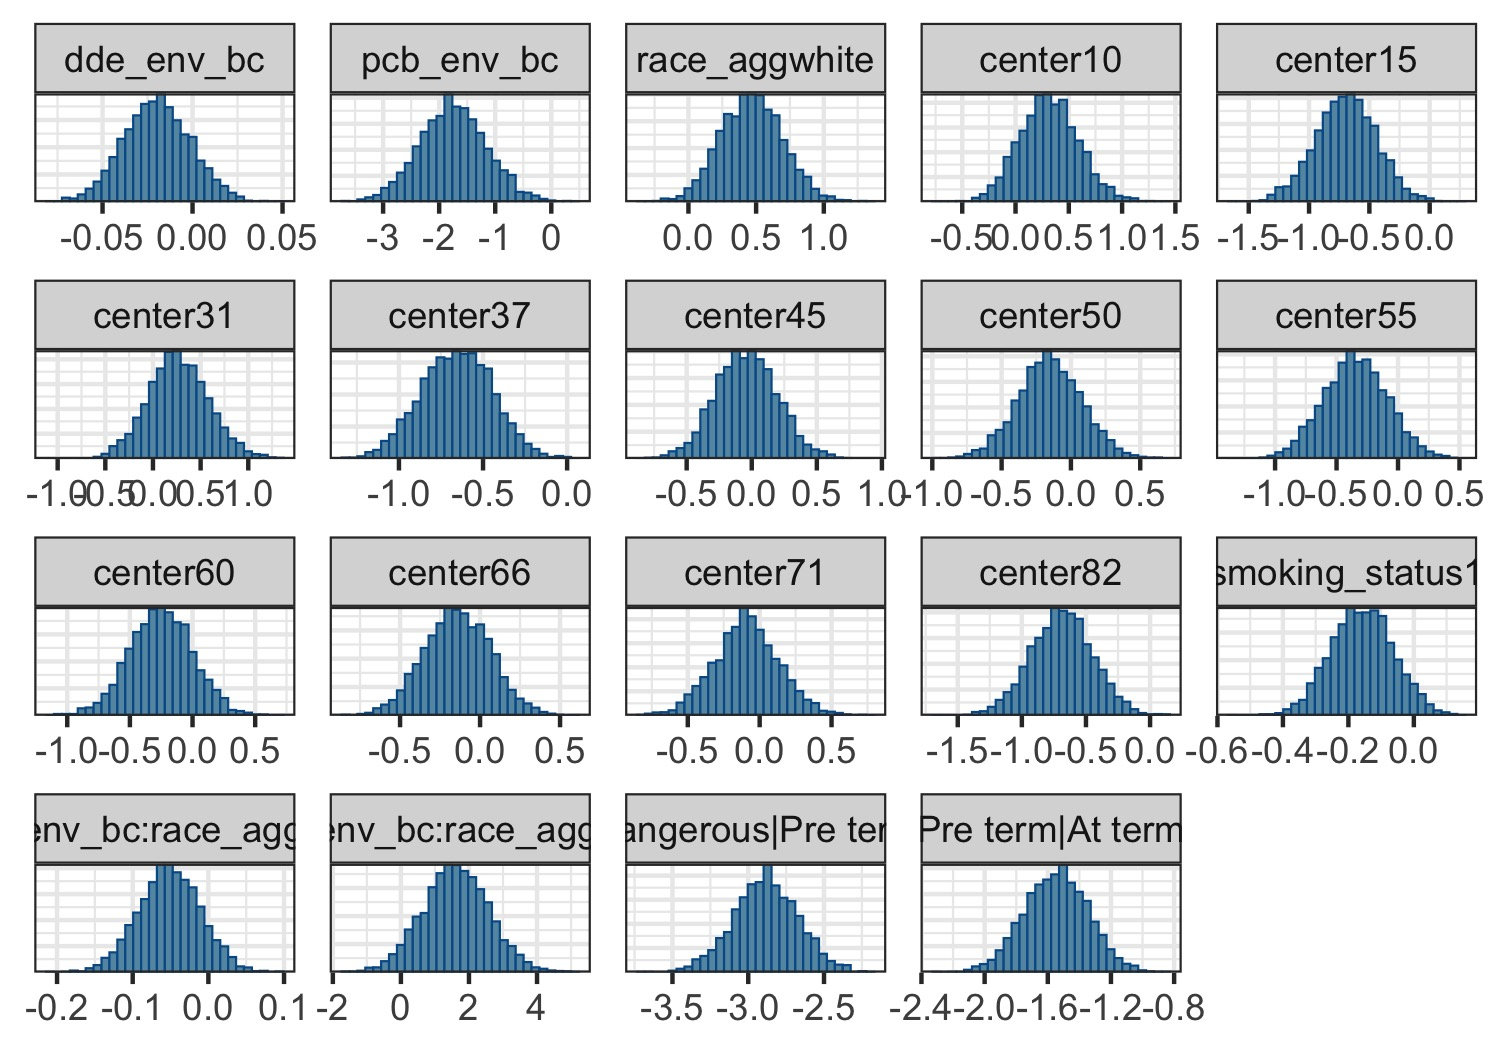
\includegraphics[width=\textwidth]{hists.jpeg}
	\caption{Histogram of 90\% credible intervals}
	\label{fig:hists}
\end{figure}

\end{document}